\documentclass[12pt]{article}


%% Including all packages that have been used in past papers.
\usepackage{graphicx}
\usepackage{amssymb}
\usepackage{amsfonts}
\usepackage{amsmath}
\usepackage{geometry}
\usepackage[bottom]{footmisc}
\usepackage{setspace}
\usepackage{caption}
\usepackage{tabularx}
\usepackage{rotating}
\usepackage{lscape}
\usepackage{version}
\usepackage{fancyhdr}
\usepackage{scalefnt}
\usepackage{booktabs}
\usepackage{threeparttable}

%%%%%%%%%   Bibliography Formatting   %%%%%%%%%

\usepackage[backend=biber,style=apa,sorting=nyt]{biblatex}% 				Bibliography will use APA formatting, and the order of the bibliography will go by author name, then year, then by title.
\addbibresource{references/bibliography.bib}%					Place the path of where the .bib file is stored that has your references.

%%%%%%%%%%%%%%%%%%%%%%%%%%%%%%%%%%%%%%%%%%%%%%%

%%%%%%%%%%  Title Page   %%%%%%%%%%%%%%%%%%%%%%

\title
{
	\underline{Rename Me with Title}
	\thanks
	{
		\noindent \underline{Replace Me Acknowledgments}
	}
}%															\Thanks{} Is a footnote that uses symbols instead of numbers and doesn't get counted with footnotes. 

\author
{
	Grant X. Storer 
	\and 
	\underline{Coauthors}
}%															If you have coauthors, use the \and command to create equal centered spacing between author and coauthor(s).
%															Optional to use the \thanks command next to each coauthor if author information to be on separate footnote lines.

\date
{
	\underline{\today}
}%															Couple of options for controlling date: 
%															\date{\today} will print the date of whenever document was last compiled.
%															\date{June, 2024} (or whatever you place in here) will print explicitly the text within the brackets.
%															\date{ } Clears out the date section to display no date.
%															All depends on where you are in the drafting stage.
%%%%%%%%%%%%%%%%%%%%%%%%%%%%%%%%%%%%%%%%%%%%%%%

\begin{document}

\maketitle%													Prints title page.

%%%%%%%%%%  Abstract   %%%%%%%%%%%%%%%%%%%%%%%%

\begin{abstract}
\underline{Enter Abstract}

\bigskip

% 															JEL Classifation line:
\noindent 	\textbf{JEL Classifications:} 
			\underline{Replace me with JEL Codes}.

% 															Keywords line:
\noindent 	\textbf{Keywords:} 
			\underline{ Replace Me with Keywords.}
\end{abstract}

%%%%%%%%%%%%%%%%%%%%%%%%%%%%%%%%%%%%%%%%%%%%%%%
\bigskip \pagebreak


\section{Template Sample}

\underline
{
	Delete Template Sample section (lines 56-89) 
	once ready for writing paper draft.
}

\subsection{Figures}

Figures are stored in the "outputs" folder. 
Do-File should export three formats of each figure and 
are stored in the following "figures" subfolders:

\begin{itemize}
	\item \textbf{eps} (best for printing)
	\item \textbf{pdf} (best overall format)
	\item \textbf{png} (best for images)
\end{itemize}


Use the following command to import figure to paper: 

\begin{figure}[ht]
	\centering
	\caption{\underline{Replace Me with Figure Title}}
	\label{fig:Replace_Me_with_Ref_Label}
	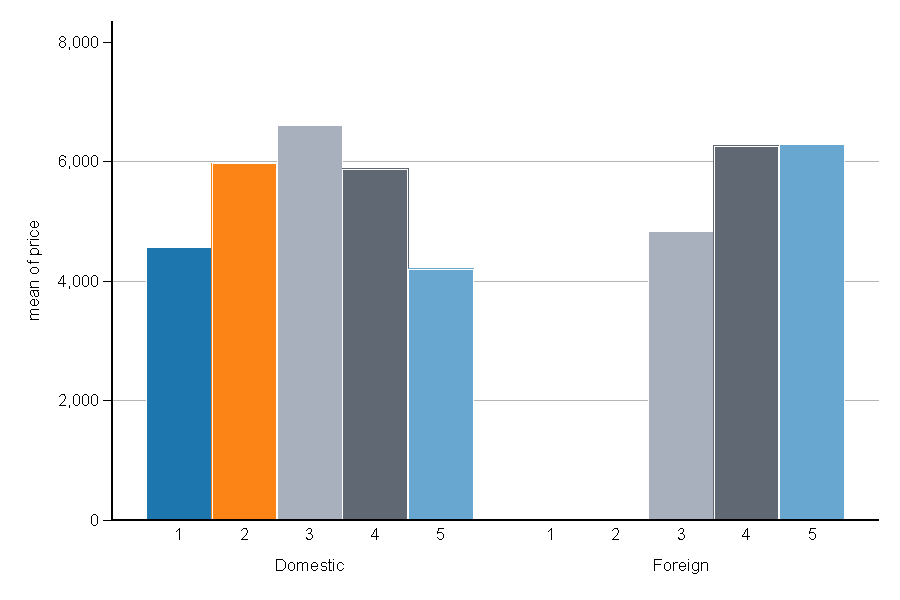
\includegraphics[width=1\textwidth]
		{outputs/figures/pdf/figure_replace_me.pdf}
\end{figure}

\subsection{Tables}

Like with Figures, 
Do-file stores tables in the "tables" subfolder of "outputs.": 

\begin{table}[htbp]\centering
\def\sym#1{\ifmmode^{#1}\else\(^{#1}\)\fi}
\caption{Car prices: Domestic vs. Foreign \label{replace\_me}}
\begin{tabular}{l*{1}{cc}}
\toprule
                    &\multicolumn{2}{c}{}     \\
                    &        Mean&          SD\\
\midrule
Domestic            &      6072.4&      3097.1\\
\addlinespace
Foreign             &      6384.7&      2621.9\\
\bottomrule
\end{tabular}
\end{table}


\subsection{Citations and References}

Citation test \parencite{storer2023sweet}. 
Figure \ref{fig:Replace_Me_with_Ref_Label} is a pdf version of 
the MPG graph, meanwhile we can also see this same graph in png format 
if we change the path name and extension name to "png." 
This graph displays prices of 
domestic\footnote
{
	"Domestic" is referring to U.S. made vehicles.\label{fnote:domestic}
} 
\& foreign vehicles, by number of repairs.

\section{Introduction}

\underline{Replace Me with Introduction}


\printbibliography%  										Note, printbibliography creates a non-numbered section, 
%															and thus don't need to enter a section command before printing bibliography.

\end{document}
